\subsubsection{Пример с двумерным массивов}

Мы будем работать с массивом типа \Tchar. Это значит, что каждый элемент требует
только одного байта в памяти.

\myparagraph{Пример с заполнением строки}
\myindex{\olly}

Заполняем вторую строку значениями 0..3:

\lstinputlisting[caption=Пример с заполнением строки,style=customc]{patterns/13_arrays/5_multidimensional/two1_RU.c}

Все три строки обведены красным. 
Видно, что во второй теперь имеются байты 0, 1, 2 и 3:

\begin{figure}[H]
\centering
\includegraphics[width=0.6\textwidth]{patterns/13_arrays/5_multidimensional/olly_2D_1.png}
\caption{\olly: массив заполнен}
\end{figure}

\myparagraph{Пример с заполнением столбца}
\myindex{\olly}

Заполняем третий столбец значениями 0..2:

\lstinputlisting[caption=Пример с заполнением столбца,style=customc]{patterns/13_arrays/5_multidimensional/two2_RU.c}

Здесь также обведены красным три строки. 
Видно, что в каждой строке, на третьей позиции, теперь записаны 0, 1 и 2.

\begin{figure}[H]
\centering
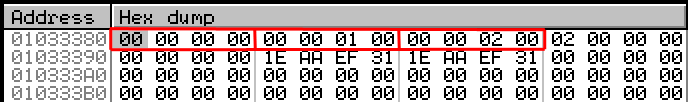
\includegraphics[width=0.6\textwidth]{patterns/13_arrays/5_multidimensional/olly_2D_2.png}
\caption{\olly: массив заполнен}
\end{figure}
